\documentclass[11pt]{article}
\usepackage[margin=1in]{geometry}
\usepackage{amssymb,amsmath,amsthm,amscd,url,hyperref,graphicx}



\newcommand{\Z}{\mathbb{Z}}
\newcommand{\Q}{\mathbb{Q}}
\newcommand{\R}{\mathbb{R}}
\newcommand{\F}{\mathbb{F}}
\newcommand{\C}{\mathbb{C}}

\DeclareMathOperator{\End}{End}

\begin{document}
\begin{center}
\Large 2015 Algebra Prelim\\
\normalsize September 14, 2015
\end{center}
\vspace{1em}

INSTRUCTIONS: Do as many of the eight problems as you can. Four completely
correct solutions will be a pass; a few complete solutions will count more than many
partial solutions. Always carefully justify your answers. If you skip a step or omit
some details in a proof, point out the gap and, if possible, indicate what would be
required to fill it in\\
\vspace{1em}

1. (a) Classify groups of order $2009 = 7^2\times 41$. 

(b) Suppose that $F$ is a field and $K/F$ is a Galois extension of degree 2009. How many intermediate fields are there -- that is, how many fields $L$ are there with $F\subset L \subset K$, both inclusions proper? (There may be several cases to consider.)\\

2. Let $K$ be a field. A discrete valuation on $K$ is a function $\nu:K\setminus\{0\}\to \Z$ such that \begin{itemize}
\item[(i)] $\nu(ab) = \nu(a)+\nu(b)$
\item[(ii)] $\nu$ is surjective 
\item[(iii)] $\nu(a+b) \ge \min \{\nu(a),\nu(b)\}$ for all $a,b\in K\setminus\{0\}$ with $a+b\neq 0$.
\end{itemize}
Let $R:=\{x\in K\setminus\{0\}\mid \nu(x)\ge 0\} \cup \{0\}$. Then $R$ is called the valuation ring of $\nu$. Prove the following 

(a) $R$ is a subring of $K$ containing the $1$ in $K$

(b) For all $x\in K\setminus\{0\}$, either $x$ or $x^{-1}$ is in $R$. 

(c) $x$ is a unit of $R$ if and only if $\nu(x) = 0$. 

(d) Let $p$ be a prime number, $K=\Q$ and $\nu_p:\Q\setminus\{0\}\to \Z$ be the function defined by $\nu_p(\frac{a}{b}) = n$ where $\frac{a}{b} = p^n\frac{c}{d}$ and $p$ does not divide $c$ and $d$. Prove that the corresponding valuation ring $R$ is the ring of all rational numbers whose denominators are relatively prime to $p$. \\

3. Let $F$ be a fieldof characteristic not equal to 2.

(a) Prove that any extension $K$ of $F$ of degree 2 is of the form $F(\sqrt{D})$ where $D\in F$ is not a square in $F$ and conversely, that each such extension has degree 2 over $F$.

(b) Let $D_1,D_2\in F$ neither of which is square in $F$. Prove that $[F(\sqrt{D_1},\sqrt{D_2}):F] = 4$ if $D_1D_2$ is not a square in $F$ and is of degree 2 otherwise. \\

4. Let $F$ be a field and $p(x) \in F[x]$ an irreducible polynomial. 

(a) Prove that there exists a field extension $K$ of $F$ in which $p(x)$ has a root.

(b) Determine the dimension of $K$ as a vector space over $F$ and exhibit a vector space basis for $K$. 

(c) If $\theta\in K$ denotes a root of $p(x)$, express $\theta^{-1}$ in terms of the basis found in part (b).

(d) Suppose $p(x) = x^3+9x+6$. Show that $p(x)$ is irreducible over $\Q$. If $\theta$ is a root of $p(x)$, compute the inverse of $1+\theta$ in $\Q(\theta)$. \\

5. Let $R$ be a ring and $Q$ an $R$-module. According to Baer’s criterion, $Q$ is
injective if and only if for every ideal $I$ of $R$, any $R$-module map $f : I \to Q$
may be extended to an $R$-module map $g : R \to Q$:
\[
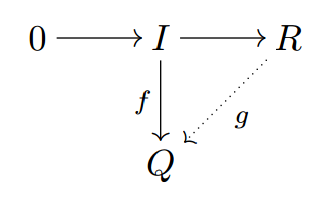
\includegraphics[width=10em]{2009.png}
\]

(a) Suppose that $p$ is prime and $n$ is a positive integer with $p$ dividing $n$.
Then multiplication makes $\Z/p\Z$ into a module over the ring $\Z/n\Z$. Show
that $\Z/p\Z$ is injective as a $\Z/n\Z$-module if and only if $p^2$ does not divide
$n$.

(b) Prove that if $R$ is a PID, then an $R$-module $Q$ is injective if and only if $rQ = Q$ for every nonzero $r\in R$. \\

6. Fix a ring $R$, an $R$-module $M$, and an $R$-module homomorphism $f:M\to M$.

(a) If $M$ satisfies the descending chain condition on submodules, show that
if $f$ is injective, then $f$ is surjective. (Hint: note that if $f$ is injective, so
are $f\circ f$, $f \circ f \circ f$, etc.)

(b) Give an example of a ring $R$, an $R$-module $M$, and an injective $R$-module
homomorphism $f : M \to M$ which is not surjective.

(c) If $M$ satisfies the ascending chain condition on submodules, show that if
$f$ is surjective, then $f$ is injective.

(d) Give an example of a ring $R$, an $R$-module $M$, and a surjective $R$-module
homomorphism $f : M \to M$ 	which is not injective.\\


7. Let $G$ be a finite group, $k$ an algebraically closed field, and $V$ an irreducible
$k$-linear representation of $G$.

(a) Show that $\mbox{Hom}_{kG}(V,V)$ is a division algebra with $k$ in its center. 

(b) Show that $V$ is finite-dimensional over $k$, and conclude that  $\mbox{Hom}_{kG}(V,V)$ is also finite-dimensional.

(c) Show the inclusion $k\to \mbox{Hom}_{kG}(V,V)$ found in (a) is an isomorphism. (For $f\in \mbox{Hom}_{kG}(V,V)$, view $f$ as a linear transformation and consider $f-\alpha I$, where $\alpha$ is an eigenvalue of $f$.)\\

8. Recall the following basic definitions and facts about ideals and varieties. Let $k$ be a field an $n$ a positive integer.
\begin{itemize}
\item if $S\subseteq k^n$, the \emph{ideal} of $S$ is $\mathcal I(S) := \{f\in k[x_1,\ldots, x_n]\mid f(s) = 0\, \forall \, s\in S\}$. $\mathcal I(S)$ is a radical ideal in $k[x_1,\ldots, x_n]$. 
\item If $I\subseteq k[x_1,\ldots, x_n]$ is an ideal, then the \emph{variety} of $I$ in $k^n$ is $\mathcal V(I) :=\{s\in k^n \mid f(s) = 0\, \forall \, f\in I\}$. 
\item If $S\subseteq k^n$, then $\mathcal V(\mathcal I(S))$ is the smallest variety containing $S$ and is called the \emph{Zariski closure} of $S$, denoted $\overline{S}$. 
\item Hilbert's Nullstellensatz: If $k$ is algebraically closed and $I$ is an ideal in $k[x_1,\ldots, x_n]$ then $\mathcal I (\mathcal V(I)) = \sqrt{I}$, where $\sqrt{I}$ is the radical of $I$.
\end{itemize}
(a) If $I$ and $J$ are ideals in $k[x_1,\ldots, x_n]$, then \emph{ideal quotient} of $I$ by $J$ is \[
I:J = \{f\in k[x_1,\ldots, x_n]\mid fg \in I\, \forall \, g\in J\}.
\]
You may use without proof the fact that $I:J$ is an ideal in $k[x_1,\ldots, x_n]$ containing $I$. Compute $\langle xz,yz\rangle :\langle z\rangle$ in $k[x,y,z]$. 

(b) Compute $\mathcal V(\langle xz, yz\rangle)$, $\mathcal V(\langle z\rangle)$ and $\mathcal V(\langle xz,yz\rangle :\langle z\rangle)$. 


(c) Let $I$ and $J$ be ideals in $k[x_1,\ldots, x_n]$. (i) Prove that $\mathcal V(I:J) \supseteq \overline{\mathcal V(I)\setminus \mathcal V(J)}$. (ii) If $k$ is algebraically closed and $I=\sqrt{I}$ then prove that $\mathcal V(I:J) = \overline{\mathcal V(I)\setminus \mathcal V(J)}$.  (Check this statement in the example from parts (a) and
(b).)



\end{document}